\documentclass[a0paper,portrait]{baposter}

\usepackage[utf8]{inputenc}

\usepackage{amsmath}    
\usepackage{amsfonts}   
\usepackage{amsthm}  
\usepackage{graphicx} 
\usepackage{xcolor}
\usepackage{relsize}


\definecolor{darktyrkis}{RGB}{0,143,149}

\begin{document}
\begin{poster}{
  columns=2,
	grid=false,
	borderColor=darktyrkis,
	headerColorOne=darktyrkis,
	headerColorTwo=darktyrkis,
	headerFontColor=white,
  headerheight=10em,
	boxColorOne=white,
  boxpadding=1em,
	headershape=rounded,
	headerfont=\Large\textsf,
	textborder=rounded,
	background=shadetb,
  bgColorOne=darktyrkis!10,
  bgColorTwo=darktyrkis!30,
	headerborder=open,
  boxshade=plain,
  eyecatcher=false
}
%%% Eye Catcher %%%%%%%%%%%%%%%%%%%%%%%%%%%%%%%%%%%%%%%%%%%%%%%%%%%%%%%%%%%%%%%
{
}
%%% Title %%%%%%%%%%%%%%%%%%%%%%%%%%%%%%%%%%%%%%%%%%%%%%%%%%%%%%%%%%%%%%%%%%%%%
{ \Huge Evolutionary optimization of machine learning pipelines}
%%% Authors %%%%%%%%%%%%%%%%%%%%%%%%%%%%%%%%%%%%%%%%%%%%%%%%%%%%%%%%%%%%%%%%%%%
{
  %\vspace{1em}
  \\Gabriela Suchopárová
}
%%% Logo %%%%%%%%%%%%%%%%%%%%%%%%%%%%%%%%%%%%%%%%%%%%%%%%%%%%%%%%%%%%%%%%%%%%%%
{
}

%%% Abstract %%%%%%%%%%%%%%%%%%%%%%%%%%%%%%%%%%%%%%%%%%%%%%%%%%%%%%%%%%%%%%%%%%
\headerbox{Abstract}{name=abstract,column=0,row=0,span=2}{
The subject of this work is the automated machine learning (AutoML), which
is a field that aims to automatize the process of model selection for a given machine
learning problem. We have developed a system that, for a given supervised
learning task represented by a dataset, finds a suitable pipeline --- combination
of machine learning, ensembles and preprocessing methods. For the search we
designed a special instance of the developmental genetic programming which enables
us to encode directed acyclic graph pipelines into a tree representation.
The system is implemented in the Python programming language and operates
on top of the scikit-learn library. The performance of our solution was tested on
72 datasets of the OpenML-CC18 benchmark with very good results.
}


% last box to reference
\headerbox{OpenML-CC18}{name=box3,column=0,span=2,above=bottom}{

\begin{minipage}{.5\textwidth}
  \centering
  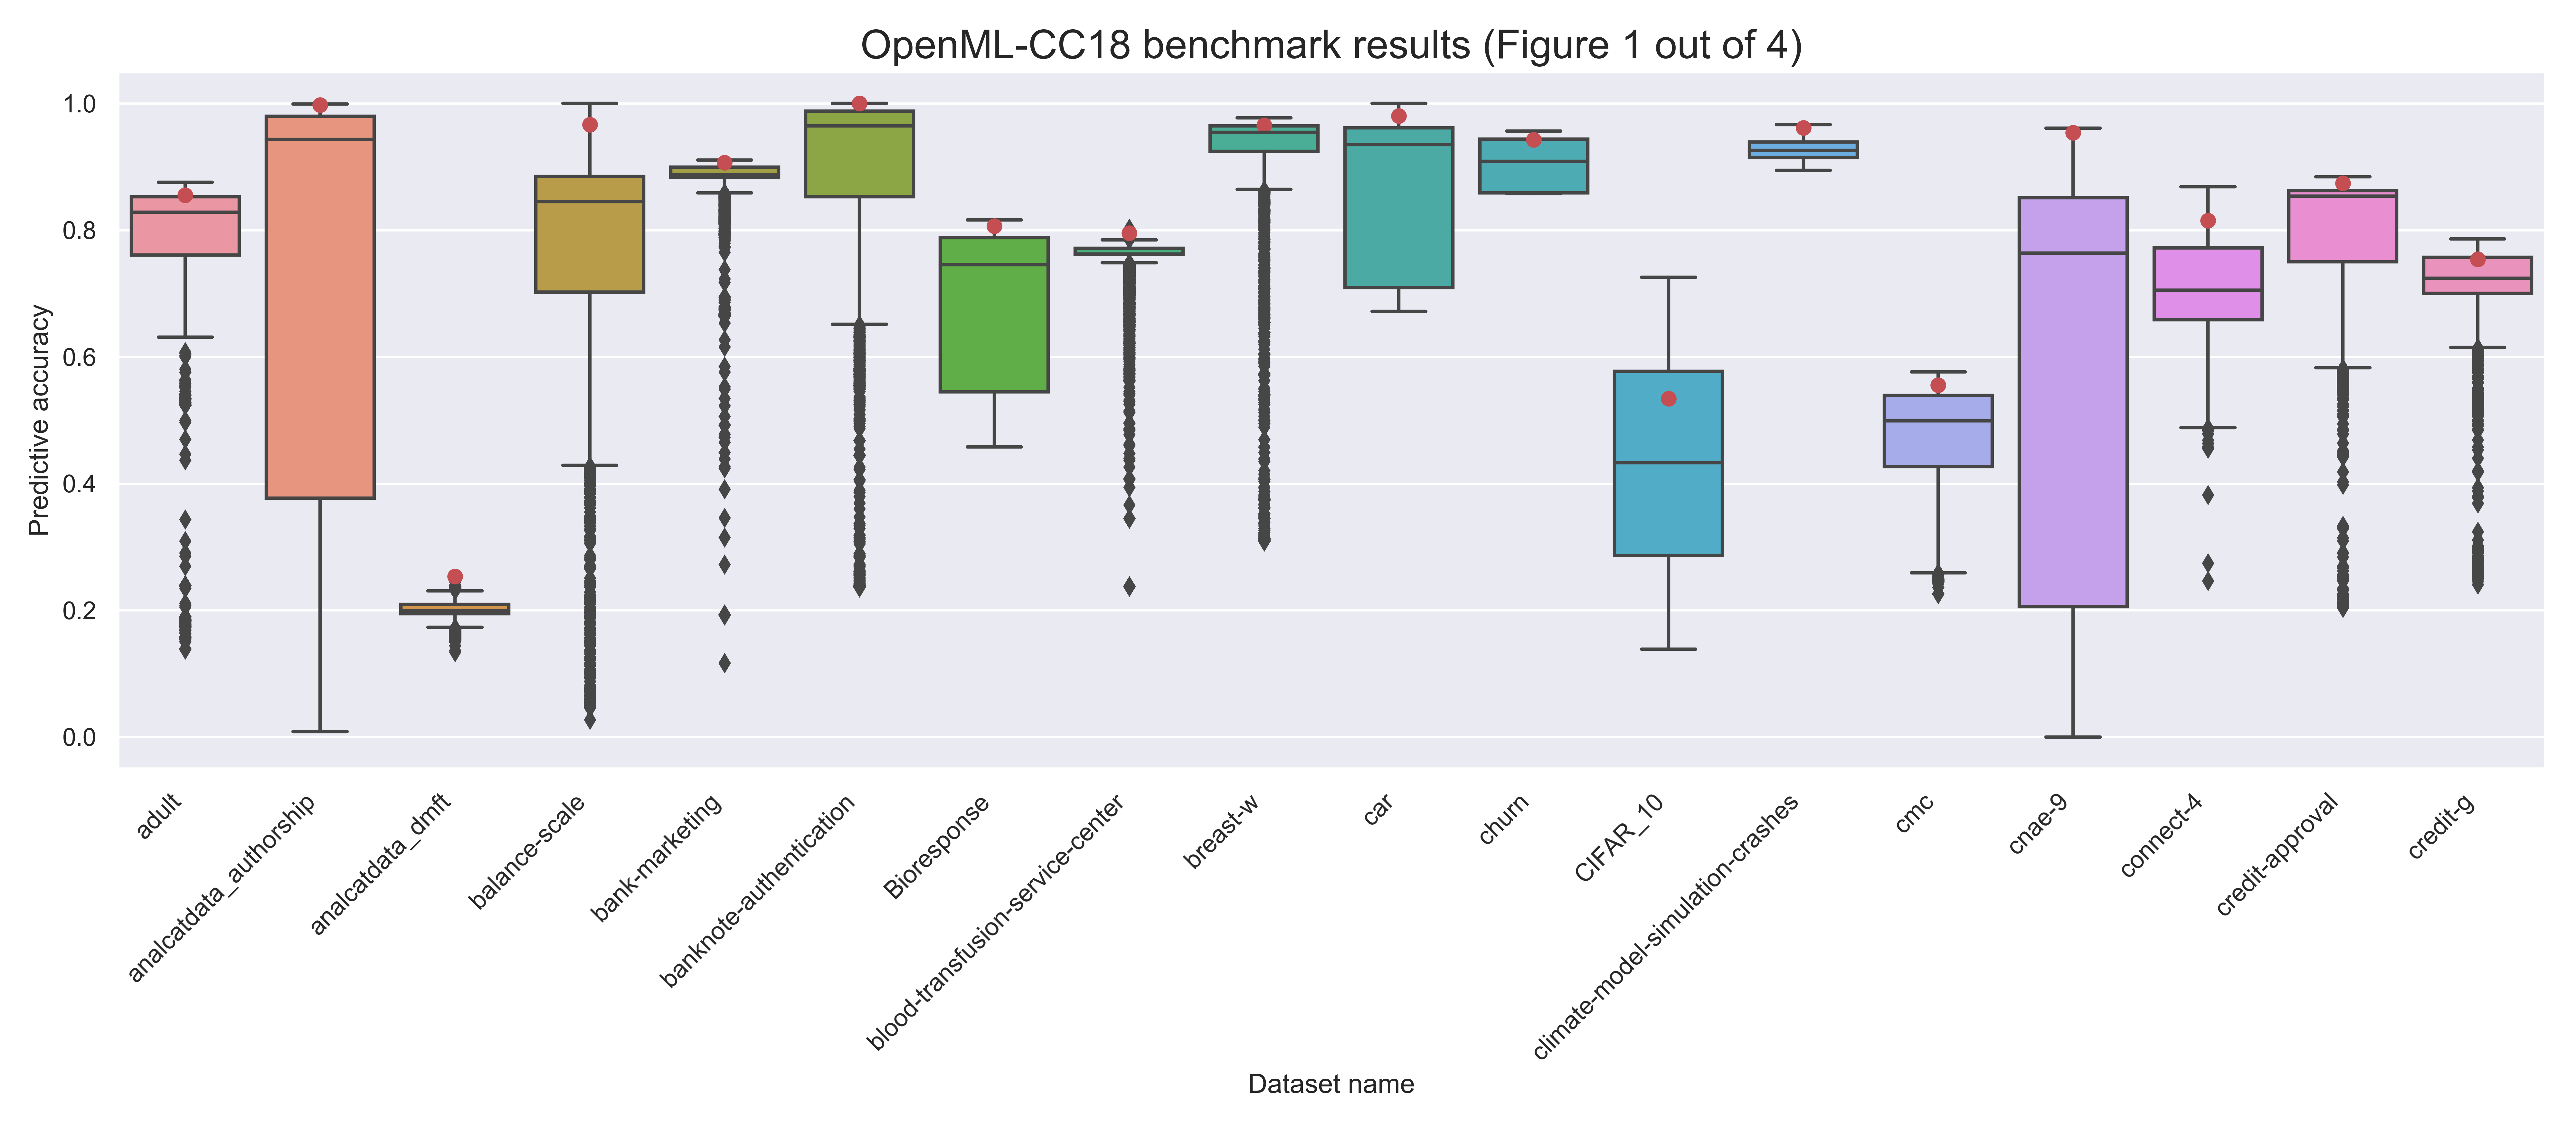
\includegraphics[width=0.9\linewidth]{../img/openml-boxplot0-hdpi.png}

\end{minipage}%
\begin{minipage}{.5\textwidth}
  \centering
  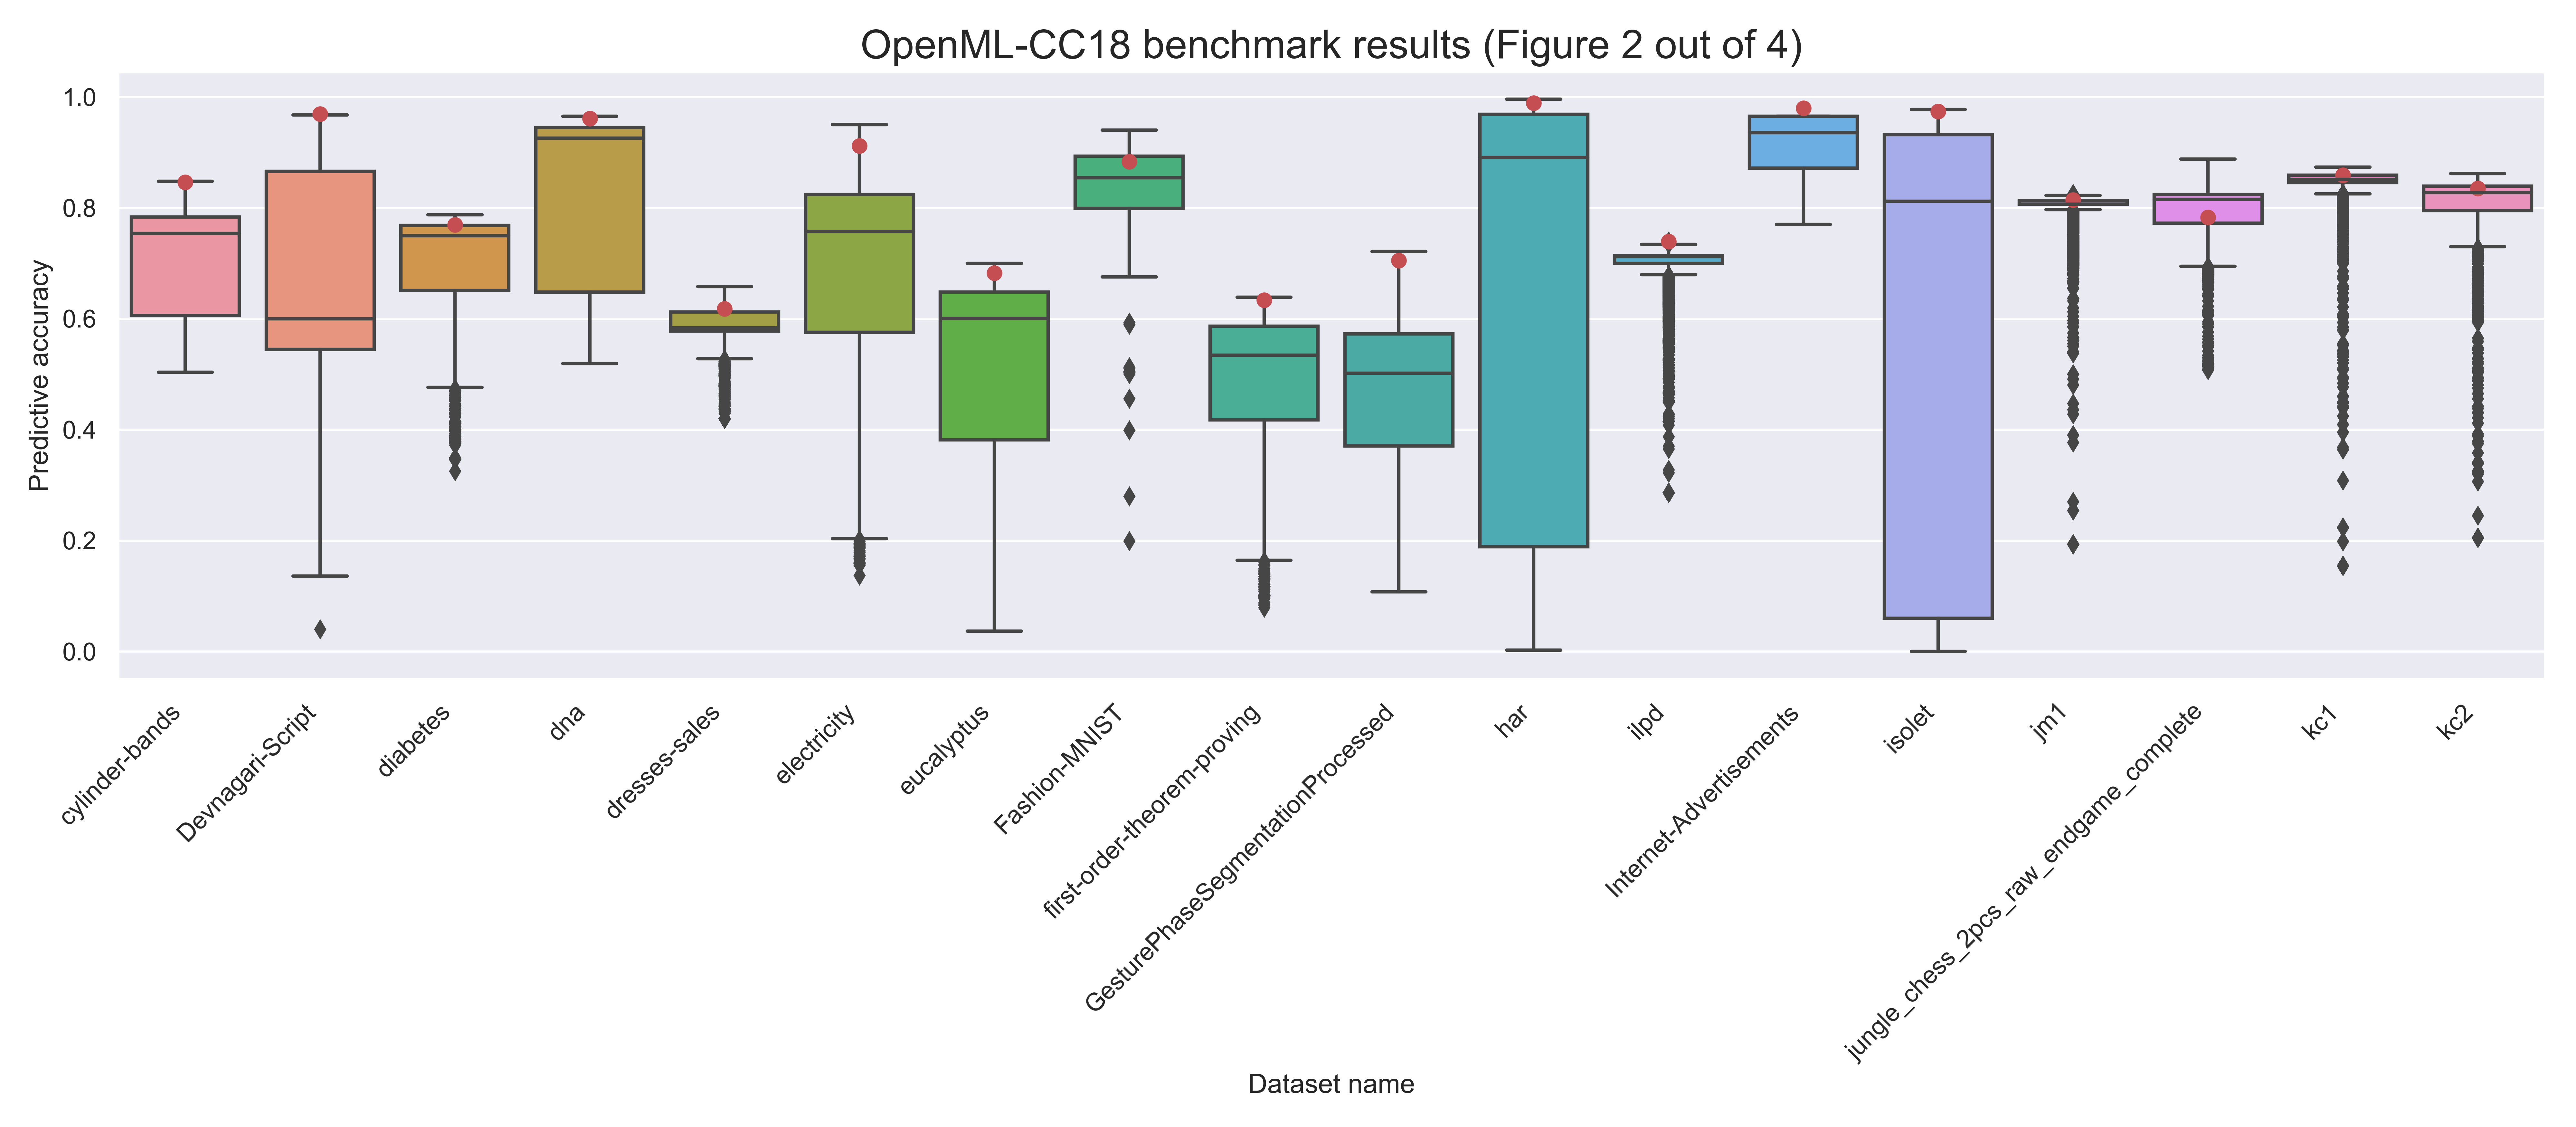
\includegraphics[width=0.9\linewidth]{../img/openml-boxplot1-hdpi.png}

\end{minipage}

\begin{minipage}{.5\textwidth}
  \centering
  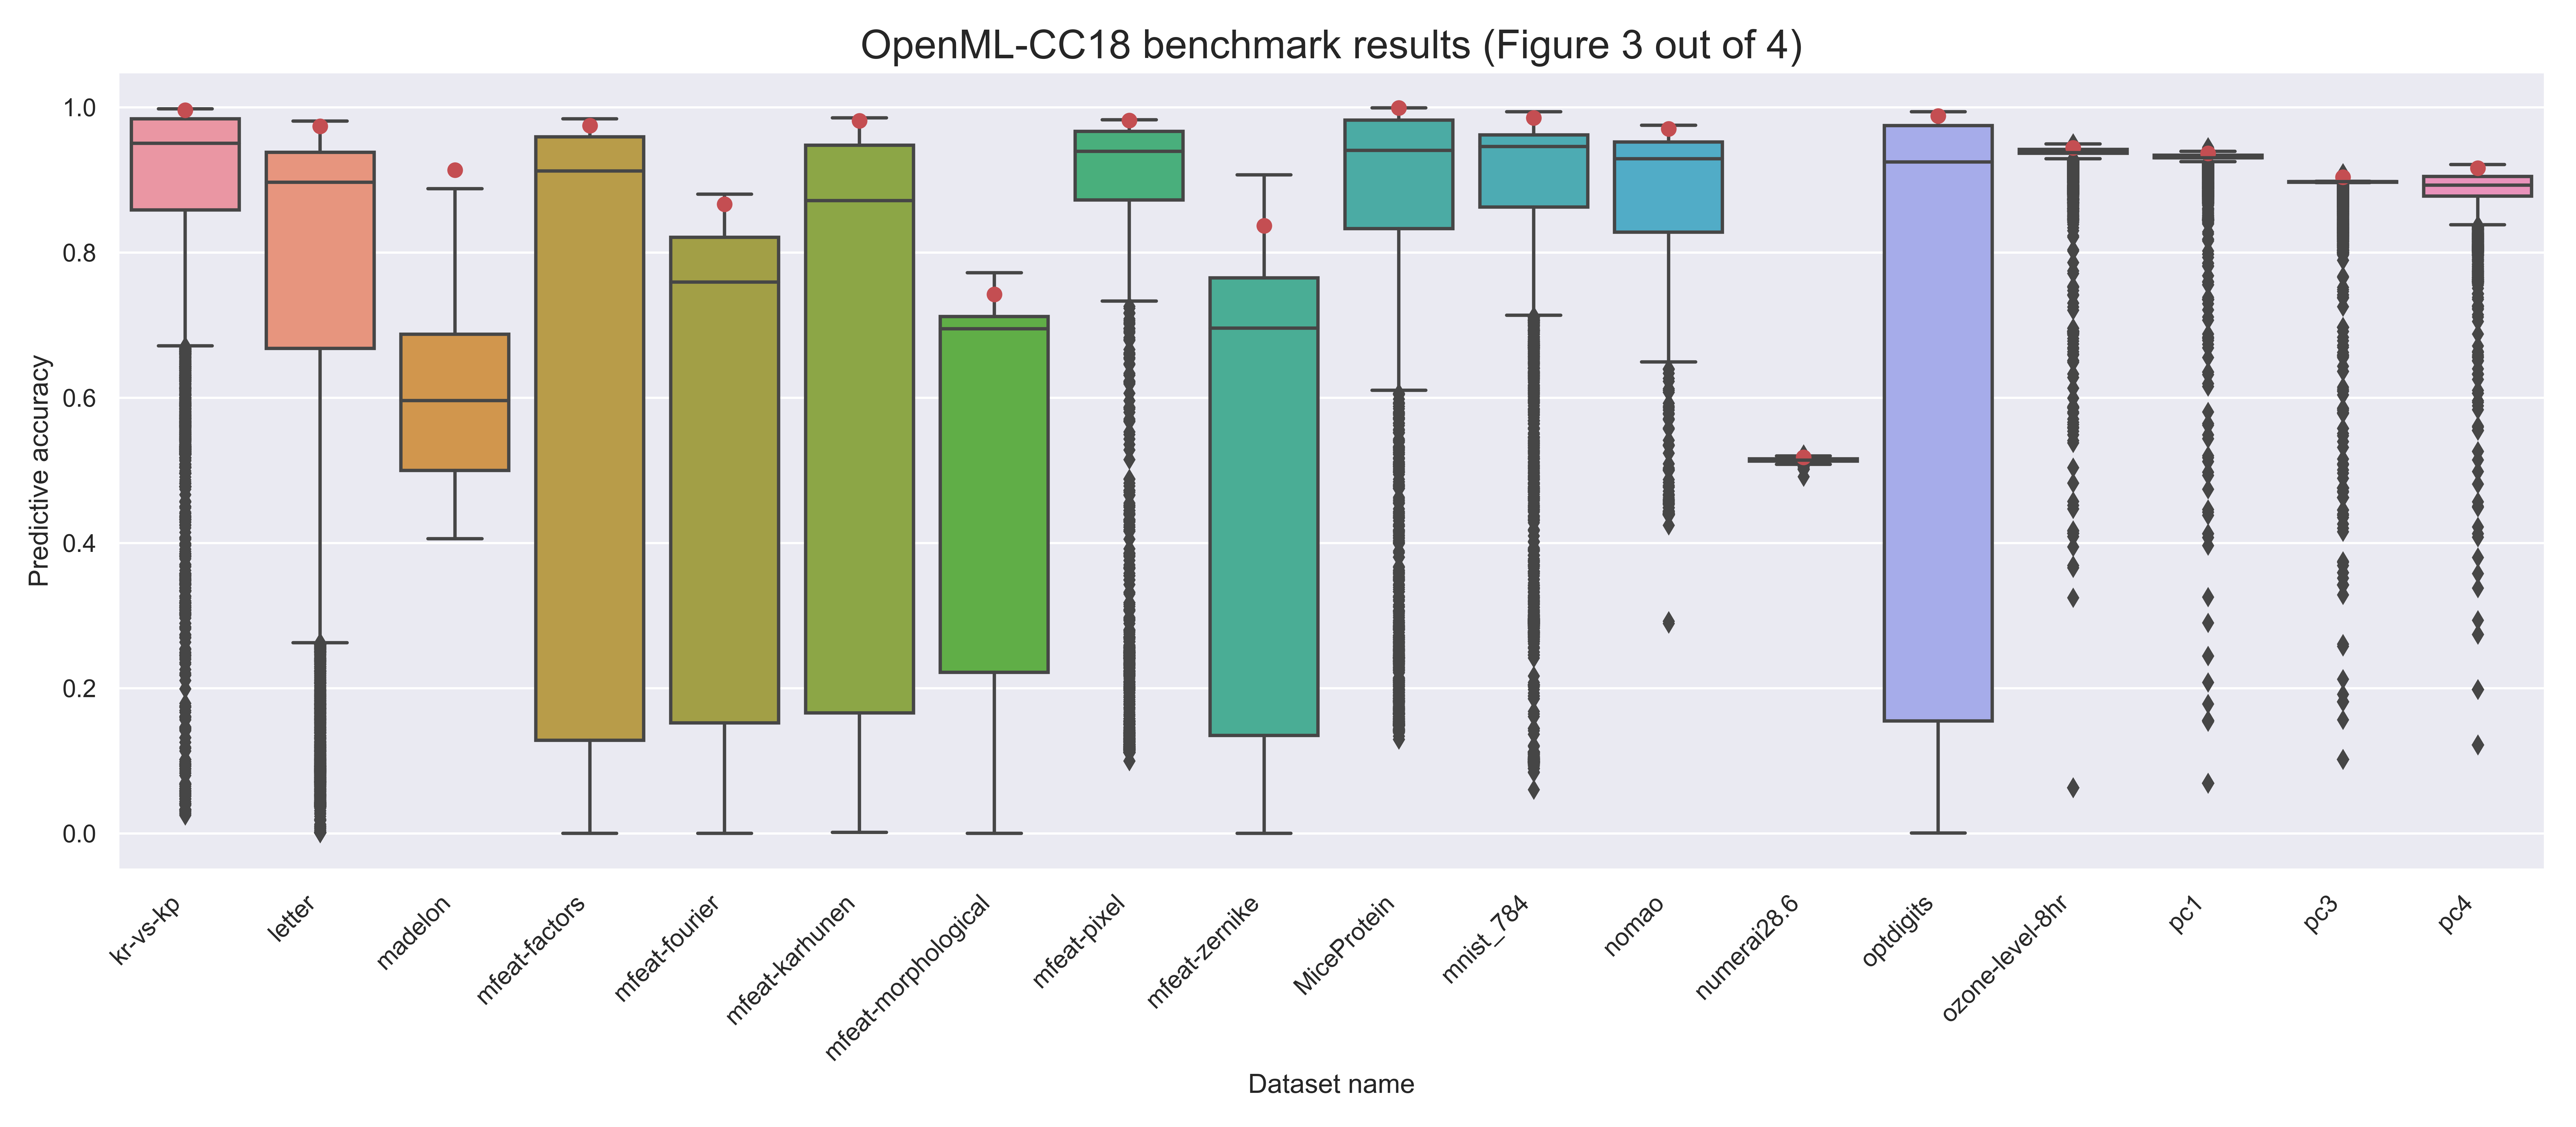
\includegraphics[width=0.9\linewidth]{../img/openml-boxplot2-hdpi.png}

\end{minipage}%
\begin{minipage}{.5\textwidth}
  \centering
  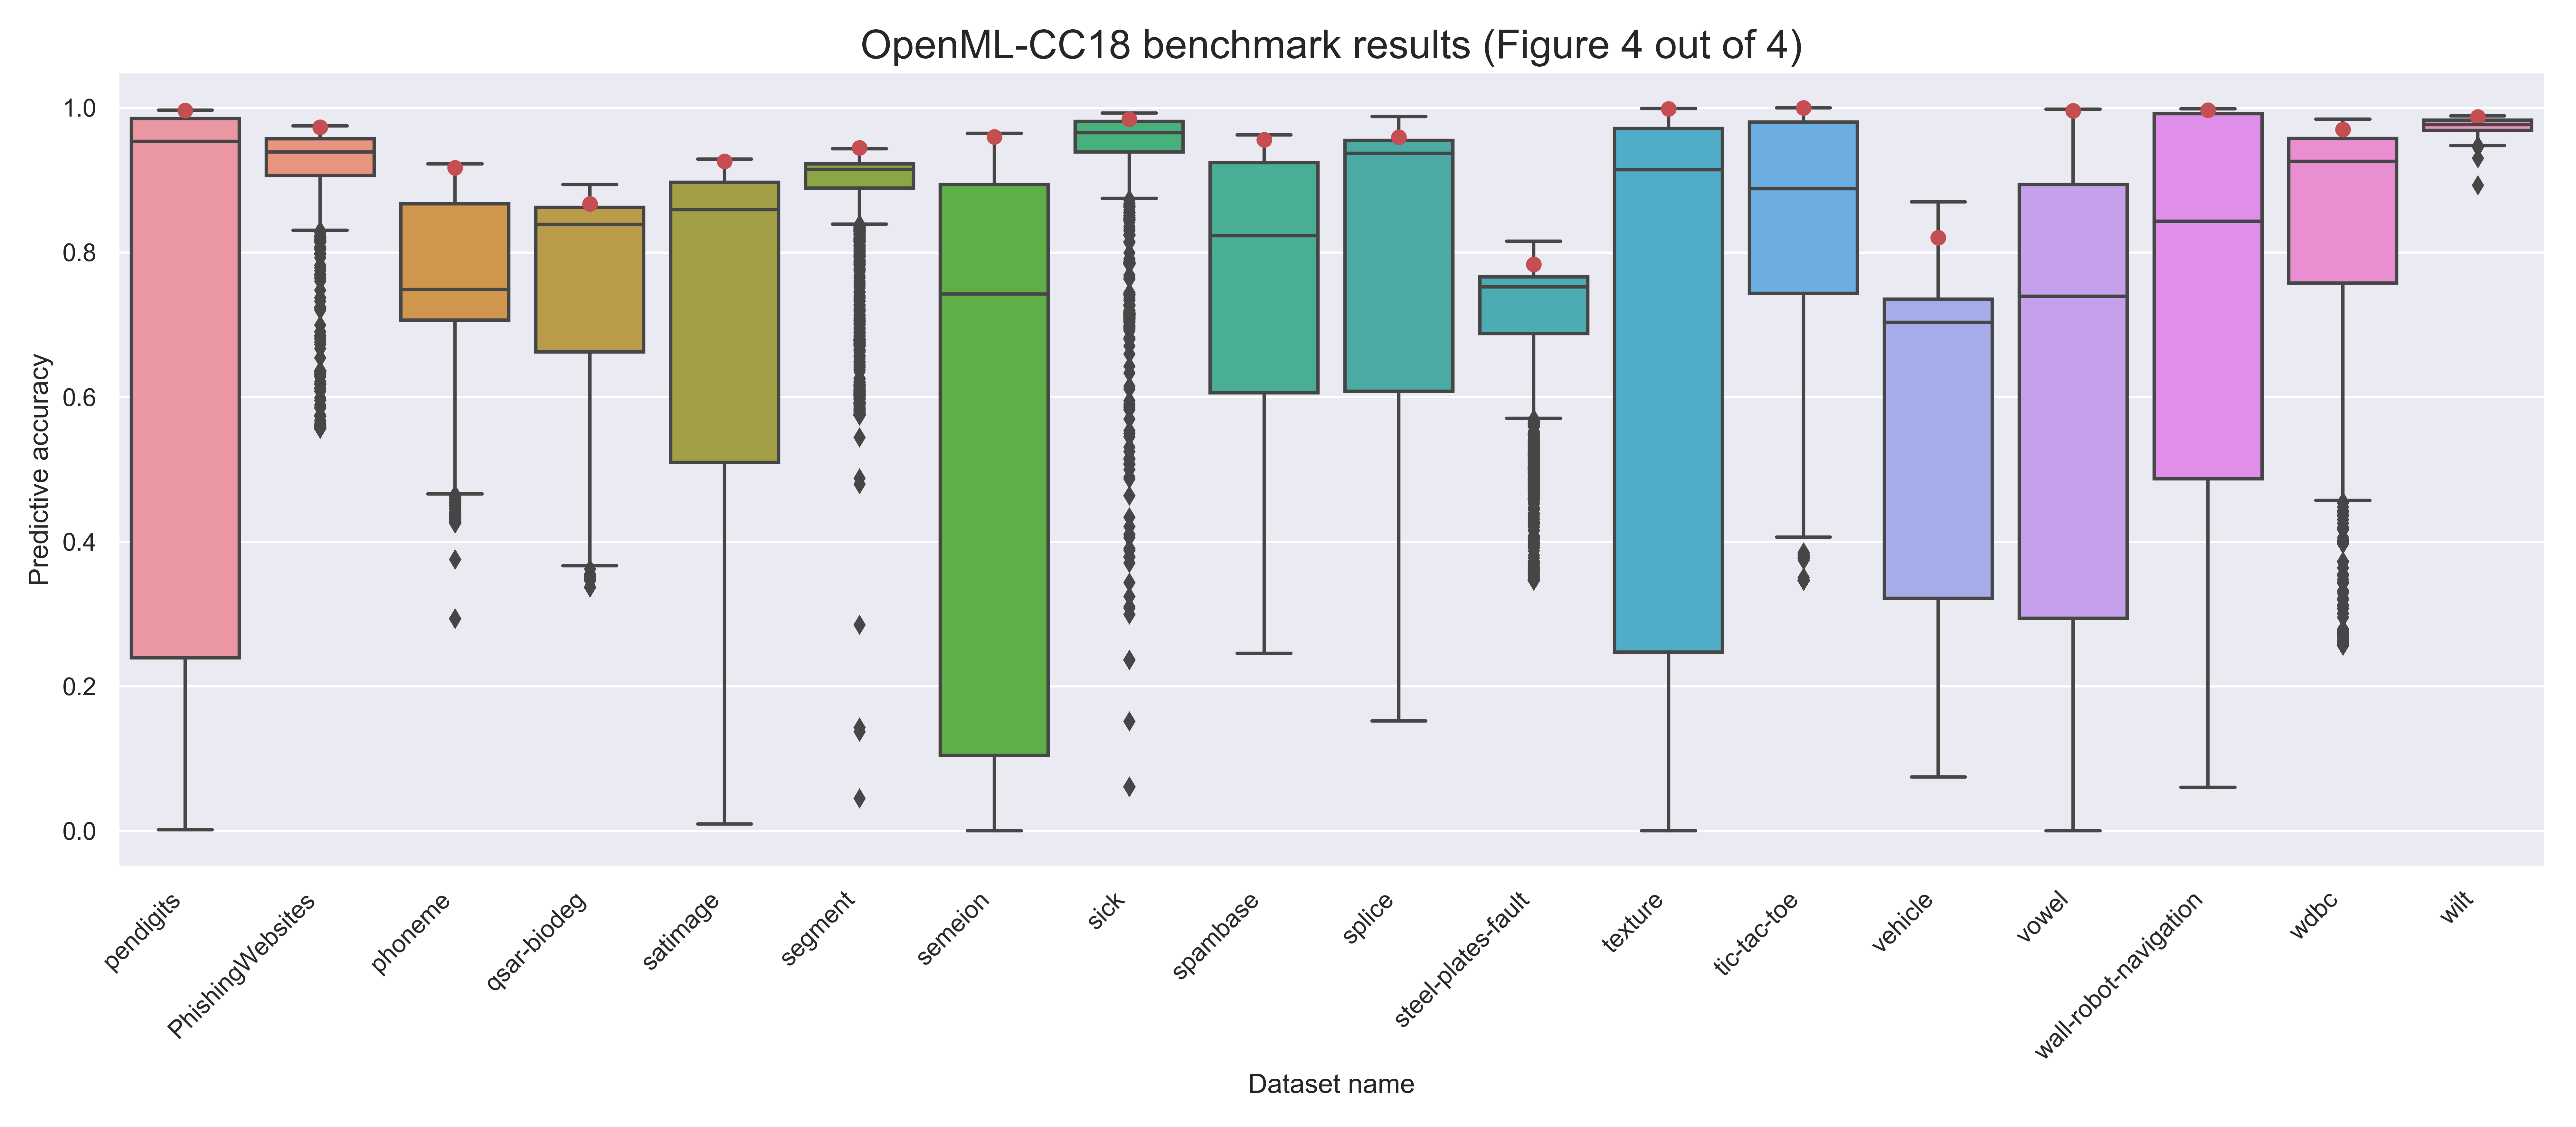
\includegraphics[width=0.9\linewidth]{../img/openml-boxplot3-hdpi.png}

\end{minipage}
}

%%% Box 1 %%%%%%%%%%%%%%%%%%%%%%%%%%%%%%%%%%%%%%%%%%%%%%%%%%%%%%%%%%%%%%%%%%%%%
\headerbox{Workflows}{name=box1,column=0,below=abstract, above=box3}{
Here will be a general workflow description.

\begin{minipage}{\textwidth}
  \centering
  \vspace{1em}
  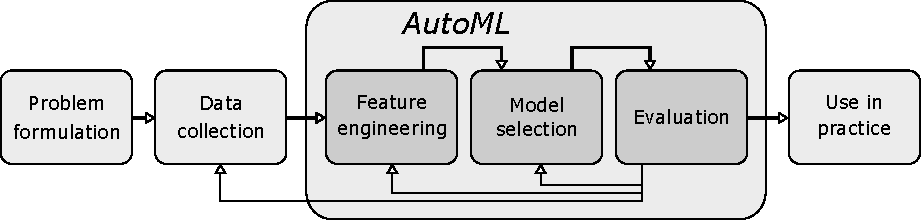
\includegraphics[width=0.9\linewidth]{../img/workflow-pdfa.pdf}
  \vspace{1em}
\end{minipage}

Existing systems focused only on\ldots

\begin{minipage}{\textwidth}
  \centering
  \vspace{1em}
  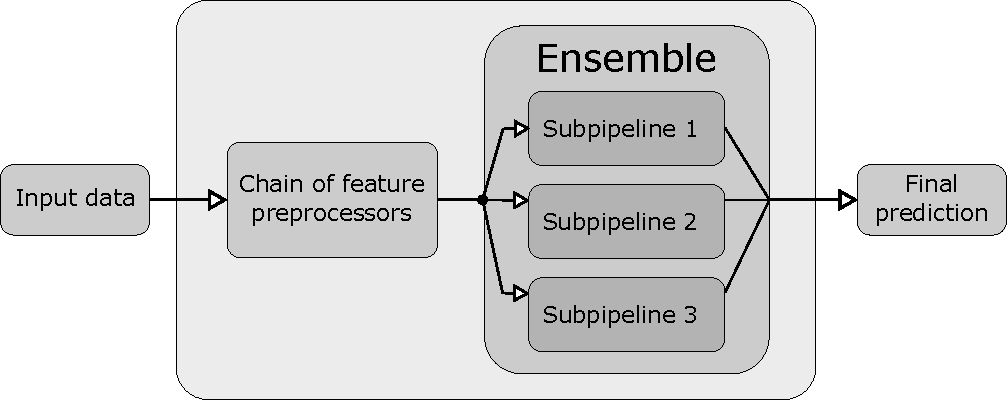
\includegraphics[width=0.7\linewidth]{../img/pipeline-pdfa.pdf}
  \vspace{1em}
\end{minipage}
}

%%% Box 2 %%%%%%%%%%%%%%%%%%%%%%%%%%%%%%%%%%%%%%%%%%%%%%%%%%%%%%%%%%%%%%%%%%%%%
\headerbox{Some Box}{name=box2,column=1,below=abstract,above=box3}{
\begin{minipage}{.5\textwidth}
  \centering
  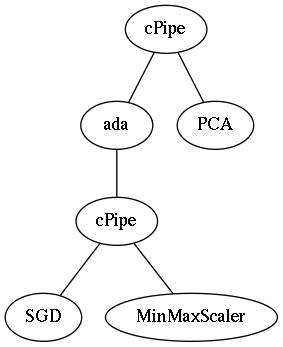
\includegraphics[width=0.5\linewidth]{../img/ada.png}

\end{minipage}%
\begin{minipage}{.5\textwidth}
  \centering
  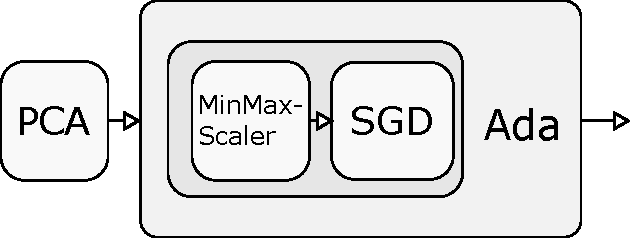
\includegraphics[width=0.9\linewidth]{../img/ada-pdfa.pdf}

\end{minipage}
\vspace{1em}

Here will be a description of pipeline-to-tree encoding.
}


\end{poster}

\end{document}